\documentclass{beamer}
%\usepackage[margin=1in]{geometry}
\usepackage{amsthm,amsmath,amsfonts,hyperref,graphicx,color,multicol}
\usepackage{enumitem,tikz}

%%%%%%%%%%
%Beamer Template Customization
%%%%%%%%%%
\setbeamertemplate{navigation symbols}{}
\setbeamertemplate{theorems}[ams style]
\setbeamertemplate{blocks}[rounded]

\definecolor{Blu}{RGB}{43,62,133} % UWEC Blue
\setbeamercolor{structure}{fg=Blu} % Titles

%Unnumbered footnotes:
\newcommand{\blfootnote}[1]{%
	\begingroup
	\renewcommand\thefootnote{}\footnote{#1}%
	\addtocounter{footnote}{-1}%
	\endgroup
}


%%%%%%%%%%
%Custom Commands
%%%%%%%%%%
\newcommand{\R}{\mathbb{R}}
\newcommand{\veca}{\vec{a}}
\newcommand{\vecb}{\vec{b}}
\newcommand{\vece}{\vec{e}}
\newcommand{\vecu}{\vec{u}}
\newcommand{\vecv}{\vec{v}}
\newcommand{\vecw}{\vec{w}}
\newcommand{\vecx}{\vec{x}}
\newcommand{\zerovector}{\vec{0}}

\newcommand{\ds}{\displaystyle}

\newcommand{\fn}{\insertframenumber}

\newcommand{\rank}{\operatorname{rank}}
\newcommand{\adj}{\operatorname{adj}}

\newcommand{\blank}[1]{\underline{\hspace*{#1}}}


%%%%%%%%%%
%Custom Theorem Environments
%%%%%%%%%%
\theoremstyle{definition}
\newtheorem{exercise}{Exercise}
\newtheorem{question}[exercise]{Question}
\newtheorem*{defn}{Definition}
\newtheorem*{exa}{Example}
\newtheorem*{disc}{Group Discussion}
\newtheorem*{nb}{Note}
\newtheorem*{recall}{Recall}
\renewcommand{\emph}[1]{{\color{blue}\texttt{#1}}}

\definecolor{Gold}{RGB}{237, 172, 26}
%Statement block
\newenvironment{statementblock}[1]{%
	\setbeamercolor{block body}{bg=Gold!20}
	\setbeamercolor{block title}{bg=Gold}
	\begin{block}{\textbf{#1.}}}{\end{block}}





\begin{document}
	\title{Math 324: Linear Algebra}
	\subtitle{Section 4.4: Linear Independence}
	\author{Mckenzie West}
	\date{Last Updated: \today}
\begin{frame}
\maketitle
\end{frame}

\begin{frame}{\insertframenumber}
	\begin{block}{\textbf{Last Time.}}
	\begin{itemize}[label=--]
		\item Linear Combination
		\item Span
	\end{itemize}
	\end{block}
	\begin{block}{\textbf{Today.}}
		\begin{itemize}[label=--]
			\item Linear Independence
		\end{itemize}
	\end{block}
\end{frame}
\begin{frame}{\fn}
\begin{exercise}
	One thing we want to avoid in a spanning set is redundancies, for example consider $S=\{(1,-1,0),(-1,1,0),(0,1,1)\}$. 
	
	A very easy redundancy check is for non-trivial solutions to:
	\[c_1\vec v_1+c_2\vec v_2+\cdots + c_k\vec v_k=\vec 0.\]
	
	Solve the homogeneous system given by
		\[c_1(1,-1,0)+c_2(-1,1,0)+c_3(0,1,1)=(0,0,0).\]
\end{exercise}
\end{frame}
\begin{frame}{\fn}
\begin{defn}
	A subset $S=\{\vec v_1,\vec v_2,\dots,\vec v_k\}$ of a vector space $V$ is called \emph{linearly independent} if the vector equation
	\[c_1\vec v_1+c_2\vec v_2+\cdots+c_k\vec v_k=\vec 0\]
	has only the trivial solution,
	\[c_1=0,\ c_2=0,\ \dots,\ c_k=0.\]
	If there are non-trivial solutions, then we call $S$ \emph{linearly~dependent}.
\end{defn}
\end{frame}
\begin{frame}{\fn}
\begin{exa}
	Is the set $S=\{1+x,1-x,2+3x,1+2x+3x^2\}$ linearly independent?
	
	Consider the homogeneous system:
	\[a(1+x)+b(1-x)+c(2+3x)+d(1+2x+3x^2)=0.\]
	Then solve for $a,b,c,d$ by considering each power of $x$:
	$$\begin{array}{rcl}\left.\begin{array}{rcrcrcrcl}
	a&+&b&+&2c&+&d&=&0\\
	a&-&b&+&3c&+&2d&=&0\\
	&&&&&&3d&=&0
	\end{array}\right\}&\rightarrow&
	\begin{bmatrix}
	1 & 1 & 2 & 1 & 0 \\
	1 & -1 & 3 & 2 & 0 \\
	0 & 0 & 0 & 3 & 0
	\end{bmatrix}
	\\&\xrightarrow{rref}&
	\begin{bmatrix}
	1 & 0 & \frac{5}{2} & 0 & 0 \\
	0 & 1 & -\frac{1}{2} & 0 & 0 \\
	0 & 0 & 0 & 1 & 0
	\end{bmatrix}.
	\end{array}$$
	Since there is a free variable in the third column, the set is linearly \textbf{dependent}.
\end{exa}
\end{frame}
\begin{frame}{\fn}
\begin{nb}[Spanning Sets and Linear Independence Tests]
	Encode each of the vectors as columns of a matrix.
	
	Row reduce the matrix.
	
	The following conclusions can be made.
	\begin{itemize}[label=--]
		\item Zero Row $\Rightarrow$ Does NOT Span the whole space
		\item Free Variable (column w/o a leading 1) $\Rightarrow$ Linearly Dependent
	\end{itemize}
\end{nb}
\end{frame}
\begin{frame}{\fn}
\begin{exercise}
	Use the guide on the previous slide to answer the following.
	\begin{enumerate}[label = (\alph*)]\setlength{\itemsep}{.15in}
		\item Is the set $S=\{(1,2),(3,4),(5,6)\}$ linearly independent? Does $S$ span $\R^2$?
		\item Is the set $S=\{(1,2,0),(3,0,4)\}$ linearly independent? Does $S$ span $\R^3$?
		\item Is the set $S=\{1,1-x-x^2,x+x^2\}$ linearly independent? Does $S$ span $P_2$?
		\item Is the set $S=\left\{
		\begin{bmatrix}1&0\\0&1\end{bmatrix},
		\begin{bmatrix}1&0\\0&-1\end{bmatrix},
		\begin{bmatrix}0&1\\1&0\end{bmatrix},
		\begin{bmatrix}0&1\\-1&0\end{bmatrix}
		\right\}$ linearly independent? Does $S$ span $M_{2}$?
	\end{enumerate}
\end{exercise}
\end{frame}
\begin{frame}{\fn}
	\vskip -.25in
\begin{statementblock}{Theorem 4.8}
	A set $S=\{\vec v_1,\vec v_2,\dots,\vec v_k\}$, $k\geq 2$, is linearly dependent if and only if at least one of the vectors $\vec v_j$ can be written as a linear combination of the other vectors in $S$.
\end{statementblock}
\begin{exa}
	Recall the linearly dependent set from the last example, $S=\{1+x,1-x,2+3x,1+2x+3x^2\}$. The row reduced matrix was $$\begin{bmatrix}
	1 & 0 & \frac{5}{2} & 0 & 0 \\
	0 & 1 & -\frac{1}{2} & 0 & 0 \\
	0 & 0 & 0 & 1 & 0
	\end{bmatrix}.$$  
	Notice that elementary row operations do not impact the relationships between the columns.	
	Therefore reading from the third column, we see $\vec v_3=\frac{5}{2}\vec v_1-\frac{1}{2}\vec v_2$, or
	\[2+3x=\frac{5}{2}(1+x)-\frac{1}{2}(1-x) \only<2->{\boxed{+0(1+2x+3x^2)}}.\]
	%\pause \fbox{Secretly, $\vec v_4$ is there too with a zero  coefficient.}
\end{exa}
\end{frame}
\begin{frame}[fragile]
\frametitle{\fn}
\begin{exercise}
	Determine whether each of the following sets is linearly independent.  If it is linearly dependent, write one of the vectors as a linear combination of the others as in the previous example.
	\begin{enumerate}[label=(\alph*)]
		\item $S=\{2-x,2x-x^2,6-5x+x^2\}$
		\item $S=\{(1,-1),(2,1)\}$
		\item $S=\{(1,-1),(2,1),(3,-2)\}$
		\item $S=\left\{
		\begin{bmatrix}1&0\\0&-2\end{bmatrix},
		\begin{bmatrix}-2&1\\1&4\end{bmatrix},
		\begin{bmatrix}0&1\\1&0\end{bmatrix}
		\right\}$
	\end{enumerate}
\end{exercise}
\end{frame}
\begin{frame}{\fn}
	\begin{block}{\textbf{Brain Break.}}
		Describe yourself in 3 words. (No, they don't have to be interview words.)
		
		\begin{center}
			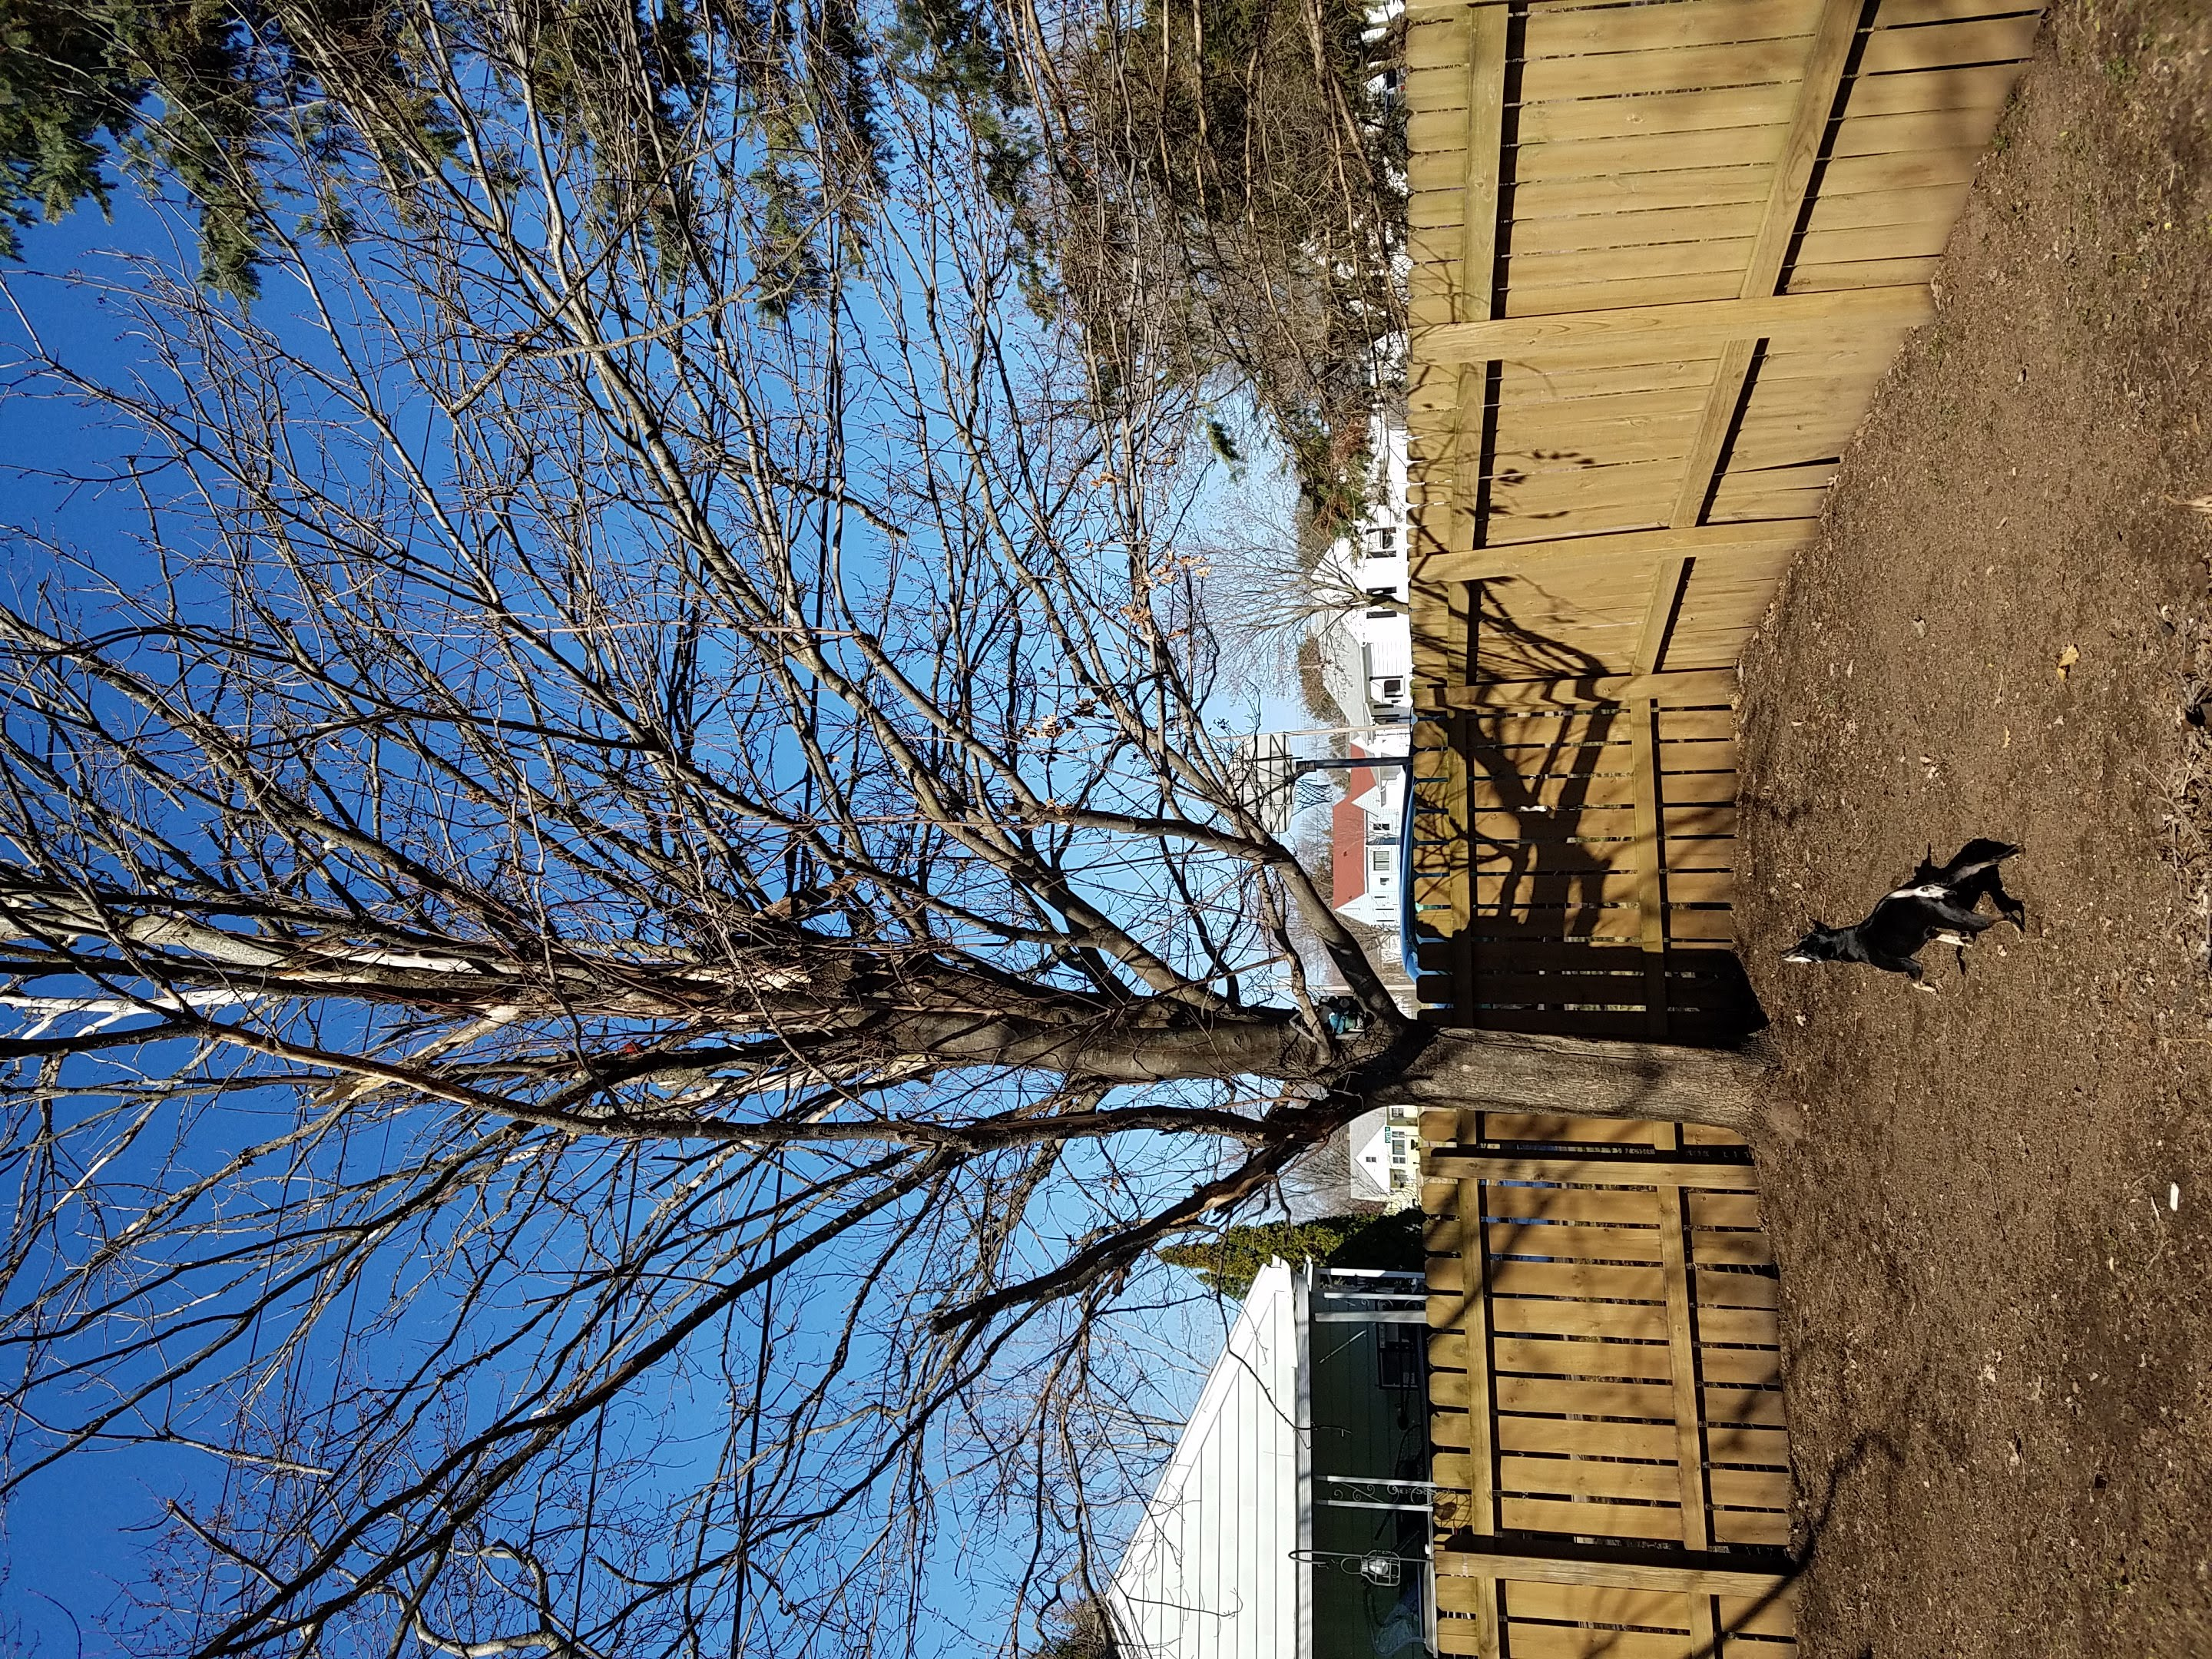
\includegraphics[angle=270,origin=c,height=1.5in]{images/bark_Pepper}
			\vskip .15in
			As I write this, Pepper is sticking with:\\
			Loud, Anti-Aviary, and Persistently-Adorable.
		\end{center}
	\end{block}
\end{frame}
\begin{frame}{\fn}
\begin{statementblock}{Corollary 4.8}
	Two vectors $\vec u$ and $\vec v$ in a vector space $V$ are linearly dependent if and only if one is a scalar multiple of the other.
\end{statementblock}
\begin{exercise}
	Explore this statement using the set $S=\{(1,2),(3,6)\}$.  How would you use the fact that $(3,6)$ is a scalar multiple of $(1,2)$ to show that there is a nontrivial way to write $\vec 0$ in terms of the vectors in $S$?
\end{exercise}
\end{frame}
\begin{frame}{\fn}
\begin{statementblock}{Corollary 4.8}
	Two vectors $\vec u$ and $\vec v$ in a vector space $V$ are linearly dependent if and only if one is a scalar multiple of the other.
\end{statementblock}
\begin{exercise}
	Prove the reverse direction of Corollary 4.8.
	\begin{proof} 
		Let $\vec u$ and $\vec v$ be vectors in a vector space $V$.  Assume that $\vec u$ is a scalar multiple of $\vec v$.
		
		Prove that $S=\{\vec u,\vec v\}$ is linearly dependent by finding $c,d$ not both zero, such that $c\vec u+d\vec v=\vec 0$.
	\end{proof}
\end{exercise}
\end{frame}
\begin{frame}{\fn}
\begin{block}{\textbf{General Method of Proving Linear Independence}}
	\begin{enumerate}[label=(\alph*)]
		\item Set up an equation of the form 
		\[c_1\vec v_1+c_2\vec v_2+\cdots+c_k\vec v_k=\vec 0.\]
		\item Show that $c_1=c_2=\cdots=c_k=0$ is the only possibility.
		\item Conclude that the set $\{\vec v_1,\vec v_2,\dots,\vec v_k\}$ is linearly independent.
	\end{enumerate}
\end{block}
\end{frame}
\begin{frame}{\fn}
\begin{exercise}
	Prove that if $S=\{\vec u,\vec v\}$ is linearly independent, then $\{\vec u+\vec v,\vec u-\vec v\}$ is linearly independent.
	
	\begin{proof}
		Let $S=\{\vec u,\vec v\}$ be a linearly independent set in a vector space $V$.  We want to show that $\{\vec u+\vec v,\vec u-\vec v\}$ is also linearly independent.  To that end, let $c,d$ be scalars such that	\[c(\vec u+\vec v)+d(\vec u-\vec v)=\vec 0.\]
		
		*Now prove that $c$ and $d$ actually have to be 0 by rearranging and using the fact that $S$ is linearly independent.*
	\end{proof}
\end{exercise}
\end{frame}
\end{document}

